\section{From Theory to Practice}
\begin{frame}{From Theory to Practice}

    \centering
    \large
    \textit{We know that \textbf{Good Data} cures Overfitting.}
    \vspace{0.5em}
    \textit{But real-world data is rarely "Good." It is messy, broken, and chaotic.}

    \vspace{1.5em}
    
    \begin{columns}[T]
        \begin{column}{0.45\textwidth}
            \centering
            \textbf{Raw Data (Reality)}
            \vspace{0.5em}
            \begin{tcolorbox}[colback=gray!10, boxrule=0pt]
                \centering \small
                \texttt{["NaN", "N/A", -500, "Cat"]}
            \end{tcolorbox}
            \small \textcolor{red}{Models crash on this.}
        \end{column}
        
        \begin{column}{0.1\textwidth}
            \centering \vspace{1cm} \Huge $\rightarrow$
        \end{column}
        
        \begin{column}{0.45\textwidth}
            \centering
            \textbf{Clean Data}
            \vspace{0.5em}
            \begin{tcolorbox}[colback=green!10, boxrule=0pt]
                \centering \small
                \texttt{[0.5, 0.2, 0.0, 1.0]}
            \end{tcolorbox}
            \small \textcolor{green!60!black}{Models learn from this.}
        \end{column}
    \end{columns}

\end{frame}

% --- SLIDE 2: EDA (EXPLORATORY DATA ANALYSIS) ---
\begin{frame}{Step 1: EDA (Know Your Data)}

    \begin{block}{Goal}
        Before training, become a \textbf{Detective}. If you feed garbage in, you get garbage out.
    \end{block}

    \vspace{1em}
    
    \begin{columns}[T]
        % Check 1: Target Dist
        \begin{column}{0.48\textwidth}
            \textbf{1. Check Target Distribution}
            \vspace{0.3em}
            \begin{tcolorbox}[colback=blue!5, boxrule=0pt]
                \centering
                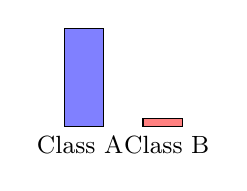
\begin{tikzpicture}[scale=0.5]
                    % Imbalanced
                    \draw[fill=blue!50] (0,0) rectangle (1,2.5); \node[below] at (0.4,0) {\small Class A};
                    \draw[fill=red!50] (2,0) rectangle (3,0.2); \node[below] at (2.6,0) {\small Class B};
                \end{tikzpicture}
                \vspace{0.5em}
                \begin{itemize}
                    \item Is it Imbalanced?
                    \item If yes, use Stratified Split \& F1-Score.
                \end{itemize}
            \end{tcolorbox}
        \end{column}
        
        % Check 2: Red Flags
        \begin{column}{0.48\textwidth}
            \textbf{2. Sanity Checks (Red Flags)}
            \vspace{0.3em}
            \begin{tcolorbox}[colback=red!5, boxrule=0pt]
                \centering
                \small
                \begin{itemize}
                    \item \textbf{Impossible Values:}
                    \item \texttt{Age: -5} $\rightarrow$ \textcolor{red}{Error?}
                    \item \texttt{Age: 200} $\rightarrow$ \textcolor{red}{Outlier?}
                    \item \textbf{Leakage:}
                    \item Does column \texttt{X} perfectly predict \texttt{y}? (e.g., "TransactionID" contains the label).
                \end{itemize}
            \end{tcolorbox}
        \end{column}
    \end{columns}
\end{frame}

% --- SLIDE 3: MISSING VALUES & SCALING ---
\begin{frame}{Step 2: Cleaning \& Scaling}

    \begin{columns}[T]
        % Missing Values
        \begin{column}{0.48\textwidth}
            \textbf{A. Missing Values (NaN)}
            \small Models cannot do math on "Empty".
            \vspace{0.5em}
            \begin{tcolorbox}[colback=gray!5, colframe=gray!50, title=Strategies]
                \small
                \begin{enumerate}
                    \item \textbf{Drop:} Delete the row (only if you have lots of data).
                    \item \textbf{Impute:} Fill with Mean/Median.
                \end{enumerate}
                \vspace{0.5em}
                \centering
                \texttt{[10, ?, 30]} $\rightarrow$ \texttt{[10, \textbf{20}, 30]}
            \end{tcolorbox}
        \end{column}
        
        % Scaling
        \begin{column}{0.55\textwidth}
            \textbf{B. Feature Scaling}
            \small Income (100k) vs. Age (50).
            \vspace{0.5em}
            \begin{tcolorbox}[colback=blue!5, colframe=blue!50, title=Why Scale?]
                \centering
                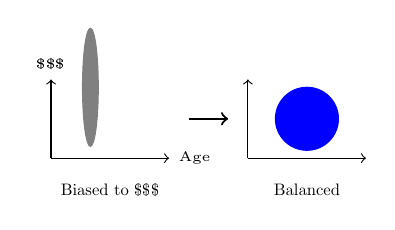
\begin{tikzpicture}[scale=0.5]
                    % Bad Scale
                    \draw[->] (0,0) -- (3,0) node[right] {\tiny Age};
                    \draw[->] (0,0) -- (0,2) node[above] {\tiny \$\$\$};
                    \filldraw[gray] (1, 1.8) ellipse (0.2 and 1.5);
                    \node[scale=0.6] at (1.5, -0.8) {Biased to \$\$\$};
                    
                    % Arrow
                    \draw[->, thick] (3.5, 1) -- (4.5, 1);
                    
                    % Good Scale
                    \draw[->] (5,0) -- (8,0);
                    \draw[->] (5,0) -- (5,2);
                    \filldraw[blue] (6.5, 1) circle (0.8);
                    \node[scale=0.6] at (6.5, -0.8) {Balanced};
                \end{tikzpicture}
                \small
                Models prioritize larger numbers. \\ Scale to $[0,1]$ (Min-Max Scaler) or \\ $\mu=0$, $\sigma=1$ (Standard Scaler).
            \end{tcolorbox}
        \end{column}
    \end{columns}
\end{frame}

% --- SLIDE 4: ENCODING & ENGINEERING ---
\begin{frame}{Step 3: Encoding \& Feature Engineering}

    \begin{columns}[T]
        % Encoding
        \begin{column}{0.48\textwidth}
            \textbf{C. Encoding (Text $\to$ Numbers)}
            \small Models speak Math, not English.
            \vspace{0.5em}
            
            \begin{tcolorbox}[colback=orange!5, boxrule=0pt]
                \textbf{1. Label Encoding} (Ordinal)
                \begin{itemize}
                    \item \texttt{["Low", "High"]} $\to$ \texttt{[0, 1]}
                    \item Use if order matters.
                \end{itemize}
                \vspace{0.3em}
                \textbf{2. One-Hot Encoding} (Nominal)
                \begin{itemize}
                    \item \texttt{["Cat", "Dog"]} $\to$
                    \item \texttt{Cat: [1, 0]}, \texttt{Dog: [0, 1]}
                    \item Use if no order exists.
                \end{itemize}
            \end{tcolorbox}
        \end{column}
        
        % Feature Engineering
        \begin{column}{0.48\textwidth}
            \textbf{D. Feature Engineering}
            \small Creating \textit{new} signals from existing data.
            \vspace{0.5em}
            
            \begin{tcolorbox}[colback=green!5, boxrule=0pt]
                \centering
                \textbf{Example: Date Object}
                \vspace{0.5em}
                
                \texttt{"2023-12-25"}
                \vspace{0.3em}
                \begin{center}
                    $\downarrow$ \textit{Extract Info} $\downarrow$
                \end{center}
                \vspace{0.3em}
                
                \begin{itemize}
                    \item \texttt{Is\_Weekend = 0}
                    \item \texttt{Month = 12} (Winter)
                    \item \texttt{Days\_To\_Holiday = 0}
                \end{itemize}
            \end{tcolorbox}
            \small \textit{This adds value that the raw date string hid.}
        \end{column}
    \end{columns}
\end{frame}

% --- PART 5: MODELING (Teaser) ---
% \section{5. Model Fitting}

% --- SLIDE 1: STEP 4 (TEASER) ---
\begin{frame}{Step 4: Fit the Model}

    \centering
    \large
    \textit{We have clean data. We have robust splits. We have metrics.}
    \vspace{0.3em} % Reduced from 0.5em
    \textbf{Now, we need a model.}
    
    \vspace{0.8em} % Adjusted spacing

    % --- Box 1: The Options ---
    \begin{tcolorbox}[colback=blue!5, colframe=blue!50, title=The Options, width=\textwidth]
        \begin{itemize}
            \item \textbf{Regression:} Linear Regression, Random Forest Regressor...
            \item \textbf{Classification:} Logistic Regression, SVM, Neural Networks...
        \end{itemize}
    \end{tcolorbox}

    \centering
    \begin{block}{}
        \centering
        We will explore \textbf{Machine Learning} \& \textbf{Deep Learning} algorithms in the next sessions!
    \end{block}

\end{frame}

% --- PART 6: SUMMARY ---
\section{References}
